\documentclass[border=4pt]{standalone}
% Preámbulo común de las figuras. Cada figura es un documento standalone
% que se compila a SVG con scripts/build_figures.sh
\usepackage[utf8]{inputenc}
\usepackage{amsmath}
\usepackage{tikz}
\usepackage[american, siunitx]{circuitikz}
\usetikzlibrary{arrows.meta,calc,decorations.pathmorphing,patterns}
\tikzset{
  >={Stealth[length=2.2mm]},
  eje/.style={->, thin},
  hilo/.style={thick},
}
% Paleta común: tonos medios legibles sobre fondo claro
\definecolor{azul}{RGB}{31,94,168}
\definecolor{rojo}{RGB}{192,57,43}
\definecolor{verde}{RGB}{39,128,73}
\definecolor{naranja}{RGB}{211,120,30}
\definecolor{morado}{RGB}{125,60,152}

\begin{document}
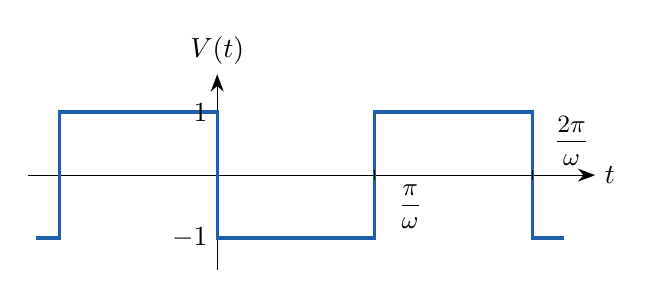
\begin{tikzpicture}[x=1.0cm, y=0.8cm]
  \draw[eje] (-2.4,0) -- (4.8,0) node[right]{$t$};
  \draw[eje] (0,-1.5) -- (0,1.6) node[above]{$V(t)$};
  \draw[very thick, azul] (-2.3,-1) -- (-2.0,-1) -- (-2.0,1) -- (0,1) -- (0,-1) -- (2,-1) -- (2,1) -- (4,1) -- (4,-1) -- (4.4,-1);
  \node[left] at (0,1) {$1$};
  \node[left] at (0,-1) {$-1$};
  \draw (2,0.08) -- (2,-0.08); \draw (4,0.08) -- (4,-0.08);
  \node[font=\small] at (2.45,-0.5) {$\dfrac{\pi}{\omega}$};
  \node[font=\small] at (4.5,0.55) {$\dfrac{2\pi}{\omega}$};
\end{tikzpicture}
\end{document}
